% ============================================================
%  High-Dimensional Option Pricing via a Hybrid Deep Galerkin–
%  Monte Carlo Framework
%  Main file — compile with: pdflatex main.tex (run twice)
% ============================================================

\documentclass[12pt, a4paper]{article}

% --- Encoding & fonts ---
\usepackage[T1]{fontenc}
\usepackage[utf8]{inputenc}

% --- Page layout ---
\usepackage[top=1in, bottom=1in, left=1in, right=1in]{geometry}

% --- Line spacing ---
\usepackage{setspace}
\onehalfspacing

% --- Math ---
\usepackage{amsmath, amssymb, amsthm}
\usepackage{mathtools}

% --- Graphics & figures ---
\usepackage{graphicx}
\usepackage{caption}
\usepackage{subcaption}
\graphicspath{{./images/}}   % put all your images in an "images/" folder

% --- Tables ---
\usepackage{booktabs}
\usepackage{array}
\usepackage{multirow}

% --- Lists ---
\usepackage{enumitem}

% --- Hyperlinks ---
\usepackage{hyperref}
\hypersetup{
    colorlinks = true,
    linkcolor  = blue,
    citecolor  = blue,
    urlcolor   = blue
}

% --- Miscellaneous ---
\usepackage{microtype}
\usepackage{xcolor}

% ============================================================
%  TITLE
% ============================================================
\title{%
    \textbf{High-Dimensional Option Pricing via a Hybrid\\
    Deep Galerkin--Monte Carlo Framework}
}
\author{}
\date{}

% ============================================================
\begin{document}

\maketitle
\thispagestyle{empty}

% ============================================================
%  ABSTRACT
% ============================================================
\begin{abstract}
High-dimensional option pricing remains a significant challenge in
computational finance due to the curse of dimensionality, which limits
the applicability of traditional mesh-based numerical methods for
solving multi-asset Black--Scholes partial differential equations.
Although Monte Carlo simulation remains the industry standard for
pricing complex derivatives, its slow convergence and high estimator
variance often result in substantial computational cost. In this work,
we propose a hybrid \textbf{Deep Galerkin Method--Monte Carlo
(DGM--MC)} framework for efficient high-dimensional option pricing,
wherein the Deep Galerkin Method is employed to learn the
Black--Scholes solution in a mesh-free setting using hard terminal
constraints, PDE residual minimization, and finance-aware sampling
strategies. The trained DGM model is subsequently integrated into
Monte Carlo simulation as a control variate to improve pricing
efficiency through variance reduction while preserving estimator
robustness. The proposed framework is validated against analytical
benchmarks, evaluated through scaling studies extending to
\textbf{100 dimensions}, and comparatively assessed against existing
approaches, including Monte Carlo--based neural regression and Deep
BSDE methods. Experimental results demonstrate competitive pricing
accuracy, improved robustness in higher-dimensional settings, and
substantial reductions in Monte Carlo estimator uncertainty,
highlighting the scalability and practical relevance of the proposed
hybrid framework for high-dimensional option pricing.

\medskip
\noindent\textbf{Keywords:} High-dimensional option pricing, Deep
Galerkin Method, Monte Carlo simulation, Control variates,
Black--Scholes PDE, Physics-informed neural networks, Variance
reduction, Computational finance
\end{abstract}

\newpage
\tableofcontents
\newpage

% ============================================================
%  SECTION 1: INTRODUCTION
% ============================================================
\section{Introduction}

\subsection{Background and Importance of Option Pricing}

Option pricing plays an important role in modern quantitative finance,
as it is crucial for derivative valuation, portfolio optimization, and
financial risk management. Options provide investors with mechanisms to
hedge against uncertainty, speculate on future market movements, and
manage financial risk exposure. Consequently, accurate pricing of
financial derivatives is essential for informed decision-making and
maintaining market efficiency.

Among the various mathematical models for derivative valuation, the
Black-Scholes model is one of the most influential approaches for
pricing financial options. By formulating the pricing problem as a
partial differential equation (PDE), the Black--Scholes framework
provides a mathematically rigorous basis for determining fair option
prices under risk-neutral assumptions. While classical single-asset
options admit analytical solutions, many practically relevant
derivatives, such as basket options and multi-asset contingent claims,
involve multiple underlying assets, significantly increasing
computational complexity and motivating the need for efficient
numerical pricing methodologies.

\subsection{Challenges in High-Dimensional Option Pricing}

Pricing multi-asset derivatives poses significant computational
challenges due to the high dimensionality of the underlying pricing
problem. In the Black-Scholes model, options on multiple underlying
assets are governed by high-dimensional partial differential equations
whose complexity increases with the number of assets. Classical
approaches, such as finite difference and finite element approaches,
become computationally heavy in such settings due to the curse of
dimensionality, where computation grows exponentially with
dimensionality. Although Monte Carlo simulation remains a widely
adopted alternative for pricing complex and high-dimensional
derivatives due to its dimension-insensitive formulation, it often
suffers from slow convergence and high estimator variance, requiring a
large number of simulations to achieve stable pricing estimates. These
kinds of limitations motivate the development of scalable and
computationally efficient alternatives capable of handling
high-dimensional derivatives.

\subsection{Existing Numerical Approaches and Their Limitations}

Several numerical methodologies have been developed for solving option
pricing problems under the Black--Scholes framework. Classical
mesh-based approaches, such as Finite Difference and Finite Element
methods, have been widely used for low-dimensional pricing problems
due to their numerical accuracy and strong mathematical foundations.
However, these approaches become computationally impractical for
high-dimensional derivatives as the discretization of the solution
domain grows exponentially with dimensionality. Monte Carlo simulation
offers a more scalable alternative and remains the industry standard
for pricing complex financial derivatives due to its flexibility in
handling high-dimensional stochastic systems. Nevertheless, its slow
convergence rate and high estimator variance often necessitate a large
number of simulation paths, resulting in increased computational
expense.

Recent advancements in deep learning have introduced neural
network-based approaches for solving high-dimensional partial
differential equations, including Physics-Informed Neural Networks
(PINNs), Deep Galerkin Methods (DGM), and Deep Backward Stochastic
Differential Equation (Deep BSDE) frameworks. In financial option
pricing, supervised approaches such as Monte Carlo-based neural
regression models have also been explored. While these methods
demonstrate promising capabilities in approximating high-dimensional
pricing functions, challenges related to computational efficiency,
scalability, and practical integration with established pricing
methodologies remain. These limitations motivate the exploration of
hybrid approaches capable of combining the learning ability of neural
PDE solvers with the robustness of traditional Monte Carlo techniques.

\subsection{Motivation for a Hybrid Deep Galerkin--Monte Carlo Framework}

Recent advancements in neural PDE solvers, particularly Deep Galerkin
Methods (DGM), have shown promising capabilities for approximating
high-dimensional option pricing functions in a mesh-free setting. By
directly learning the solution of the partial differential equation
via automatic differential and residual minimization, DGM provides an
efficient alternative to classical mesh-based solvers in
high-dimensional environments. However, despite their flexibility and
approximation capability, neural network-based pricing frameworks are
often difficult to adopt as standalone replacements for established
numerical methods in practical financial settings, where robustness,
interpretability, and reliability remain essential considerations.

In contrast, Monte Carlo simulation remains the industry standard for
pricing multi-asset derivatives due to its theoretical robustness and
flexibility across diverse payoff structures. Despite all this, the
slow convergence rate and high estimator variance associated with
Monte Carlo methods often impose substantial computational costs,
particularly in high-dimensional settings. Motivated by the
complementary strengths of both approaches, this work proposes a
hybrid Deep Galerkin--Monte Carlo (DGM--MC) framework in which a
trained DGM model is integrated into a Monte Carlo simulation as a
control variate. The central objective is not to replace Monte Carlo
estimation, but rather to enhance its computational efficiency through
variance reduction while preserving its reliability for practical
option pricing applications.

\subsection{Contributions of the Present Work}

The primary contribution of this work is the development of a
\textbf{hybrid Deep Galerkin Method--Monte Carlo (DGM--MC) framework}
for high-dimensional option pricing, wherein a trained DGM model is
incorporated into Monte Carlo simulation as a control variate to
improve computational efficiency through variance reduction. Rather
than replacing Monte Carlo simulation, the proposed framework
complements it by enhancing estimator efficiency while preserving the
robustness and practical reliability of stochastic pricing methods in
financial applications. The key contributions of this work are
summarized as follows:

\begin{itemize}

    \item \textbf{A hybrid DGM--Monte Carlo framework is proposed for
    high-dimensional option pricing}, integrating a trained Deep
    Galerkin Method with Monte Carlo simulation through a control
    variate formulation to reduce estimator uncertainty while
    preserving pricing consistency.

    \item \textbf{A mesh-free DGM-based PDE learning framework is
    developed} for solving high-dimensional multi-asset Black--Scholes
    equations using hard terminal constraints, PDE residual
    minimization, and finance-aware sampling strategies to improve
    approximation quality in financially relevant regions of the state
    space.

    \item \textbf{The proposed methodology is systematically validated
    through analytical benchmarking, scaling analysis, ablation
    studies, and Greeks estimation}, enabling comprehensive evaluation
    of pricing accuracy, optimization stability, and model robustness
    across increasing dimensionality.

    \item \textbf{A comparative performance study is conducted against
    existing approaches}, including Monte Carlo--based neural
    regression and Deep BSDE methods, with experimental evaluation
    extending to dimensions as high as \textbf{100}, demonstrating
    competitive pricing accuracy in moderate dimensions and improved
    robustness in higher-dimensional settings.

    \item \textbf{A hybrid variance reduction mechanism is empirically
    evaluated}, demonstrating substantial reductions in Monte Carlo
    estimator uncertainty and highlighting the practical relevance of
    the proposed framework for computationally efficient
    high-dimensional option pricing.

\end{itemize}

\subsection{Organization of the Paper}

The remainder of this paper is organized as follows. Section 2
presents the mathematical formulation of the high-dimensional option
pricing problem under the Black--Scholes framework. Section 3
introduces the Deep Galerkin Method framework, including the proposed
constraint formulation, sampling strategies, and optimization
procedure. Section 4 presents the proposed hybrid Deep
Galerkin--Monte Carlo framework and its variance reduction mechanism.
Section 5 describes the experimental setup and evaluation
methodology. Section 6 discusses the numerical experiments, including
validation, scaling analysis, ablation studies, Greeks estimation,
hybrid Monte Carlo performance, and comparative benchmarking. Finally,
Section 7 concludes the paper and outlines directions for future
research.

% ============================================================
%  SECTION 2: Mathematical Background and Problem Formulation
% ============================================================

\section{Mathematical Background and Problem Formulation}

\subsection{Multi-Asset Black--Scholes PDE}

Consider a financial market consisting of \textbf{d underlying assets},
whose prices evolve according to correlated stochastic processes under
the risk-neutral measure. Let

\[
    \mathbf{S}(t) = \bigl(S_1(t),\ S_2(t),\ \ldots,\ S_d(t)\bigr)
\]

represent the vector of underlying asset prices at time \textbf{t},
where each asset follows a geometric Brownian motion. The objective is
to determine the fair value of a European-style derivative whose payoff
depends on multiple underlying assets.

Under the Black--Scholes framework, the option price function
$V(\mathbf{S},t)$ satisfies the following \textbf{d-dimensional
Black--Scholes partial differential equation}:

\begin{equation}
    \frac{\partial V}{\partial t}
    + \frac{1}{2} \sum_{i=1}^{d} \sum_{j=1}^{d}
      \rho_{ij}\, \sigma_i\, \sigma_j\, S_i\, S_j\,
      \frac{\partial^2 V}{\partial S_i \partial S_j}
    + r \sum_{i=1}^{d} S_i \frac{\partial V}{\partial S_i}
    - rV = 0
    \label{eq:bs_pde}
\end{equation}

Where:
\begin{itemize}
    \item $r$ denotes the risk-free interest rate,
    \item $\sigma_i$ represents the volatility of the $i$-th asset, and
    \item $\rho_{ij}$ denotes the correlation between assets $S_i$ and
          $S_j$.
\end{itemize}

The second-order mixed-derivative terms capture the dependency
structure among correlated assets and significantly increase
computational complexity as the dimensionality increases.

The pricing problem is supplemented with a \textbf{terminal payoff
condition} at maturity $T$:

\[
    V(\mathbf{S},\, T) = \Phi(\mathbf{S})
\]

where $\Phi(\mathbf{S})$ represents the payoff function of the
derivative contract. Therefore, the objective of the pricing problem is
to approximate the option price function $V(\mathbf{S},t)$ that
satisfies both the governing partial differential equation and the
associated terminal condition.

\subsection{Risk-Neutral Asset Dynamics}

Under the risk-neutral framework, the price dynamics of the underlying
assets are assumed to follow correlated geometric Brownian motion
processes. For the $i$-th asset, the stochastic evolution is governed
by:

\begin{equation}
    dS_i(t) = r\, S_i(t)\, dt + \sigma_i\, S_i(t)\, dW_i(t),
    \qquad i = 1, 2, \ldots, d
    \label{eq:gbm}
\end{equation}

Where:
\begin{itemize}
    \item $S_i(t)$ denotes the price of the $i$-th asset at time $t$,
    \item $r$ represents the constant risk-free interest rate,
    \item $\sigma_i$ denotes the volatility of the $i$-th asset, and
    \item $W_i(t)$ represents a standard Brownian motion process.
\end{itemize}

To model dependency among assets, the Brownian motions are assumed to
be correlated, such that:

\[
    \mathrm{Corr}\!\left(dW_i(t),\, dW_j(t)\right) = \rho_{ij}
\]

where $\rho_{ij}$ denotes the correlation coefficient between assets
$i$ and $j$. This correlation structure introduces mixed derivative
terms in the multi-dimensional Black--Scholes PDE and increases the
complexity of solving the pricing problem as the number of underlying
assets increases.

Under the risk-neutral measure, the expected growth of asset prices is
governed by the risk-free rate rather than the actual market return.
This assumption forms the basis for deriving the Black--Scholes pricing
equation and enables consistent valuation of derivative contracts
through no-arbitrage principles.

\subsection{Option Payoff Formulation}

The proposed framework is designed to price European-style multi-asset
derivatives whose payoffs depend on multiple underlying assets. In this
work, the \textbf{arithmetic basket call option} serves as the primary
pricing problem. While additional payoff structures are incorporated
for validation and benchmarking purposes.

For a \textbf{European arithmetic basket call option}, the payoff at
maturity is given by:

\begin{equation}
    \Phi(\mathbf{S}) = \max\!\left[
        \frac{1}{d} \sum_{i=1}^{d} S_i - K,\; 0
    \right]
    \label{eq:arith_basket}
\end{equation}

Where:
\begin{itemize}
    \item $S_i$ denotes the price of the $i$-th underlying asset at
          maturity,
    \item $d$ represents the number of underlying assets, and
    \item $K$ denotes the strike price.
\end{itemize}

The arithmetic basket option constitutes the principal benchmark in
this study due to its practical relevance in financial markets and the
absence of closed-form analytical solutions in higher dimensions,
thereby requiring numerical approximation techniques.

To validate model accuracy, a \textbf{geometric basket call option} is
additionally considered, whose payoff is defined as:

\begin{equation}
    \Phi(\mathbf{S}) = \max\!\left[
        \left(\prod_{i=1}^{d} S_i\right)^{1/d} - K,\; 0
    \right]
    \label{eq:geom_basket}
\end{equation}

Unlike arithmetic basket options, geometric basket options admit
analytical solutions under the Black--Scholes framework, making them
suitable for validating the correctness of the proposed methodology.

Furthermore, the framework supports additional multi-asset payoff
structures, including \textbf{maximum call options}, defined as:

\begin{equation}
    \Phi(\mathbf{S}) = \max\!\left[
        \max(S_1, S_2, \ldots, S_d) - K,\; 0
    \right]
    \label{eq:max_call}
\end{equation}

and \textbf{spread options}, defined as:

\begin{equation}
    \Phi(\mathbf{S}) = \max\!\left(S_1 - S_2 - K,\; 0\right)
    \label{eq:spread}
\end{equation}

These additional payoff formulations demonstrate the flexibility of the
proposed framework in handling diverse multi-asset derivative pricing
problems.

\subsection{Curse of Dimensionality in Option Pricing}

One of the most significant challenges in the multi-asset pricing
arises from the curse of dimensionality, in which the computational
cost increases rapidly with the number of underlying assets. Under the
Black--Scholes model, the pricing of a derivative involving $d$ assets
requires solving a $d$-dimensional PDE, resulting in a rapidly
increasing solution domain as dimensionality increases.

Classical mesh-based numerical methods, such as Finite Difference and
Finite Element techniques, rely on discretizing the solution domain
into computational grids. If $n$ discretization points are assigned to
each dimension, the total number of grid points grows proportionally to

\[
    \mathcal{O}(n^d)
\]

where $d$ denotes dimensionality. Consequently, even moderate increases
in the number of assets can result in prohibitively high computational
requirements. For example, assigning 100 grid points per dimension
yields $100^{10}$ grid points in a ten-dimensional problem, rendering
classical discretization-based approaches computationally infeasible.

Although Monte Carlo methods partially solve the problem of
dimensionality by using dimension-insensitive simulation strategies.
But the slow convergence rate often requires a large number of
simulation paths for stable option pricing estimates. These challenges
motivate the exploration of mesh-free learning approaches, such as DGM,
which avoids explicit domain discretization and instead learns the
solution directly through PDE-constrained optimization.

% ============================================================
%  SECTION 3: Deep Galerkin Method Framework
% ============================================================

\section{Deep Galerkin Method Framework}

\subsection{Motivation for the Deep Galerkin Method}

The computational challenges associated with high-dimensional option
pricing motivate the need for numerical methods that overcome the curse
of dimensionality without relying on explicit domain discretization.
While classical mesh-based methods become computationally infeasible in
higher dimensions, neural network-based PDE solvers offer a promising
alternative by directly approximating the solution function via
optimization.

Among these approaches, the \textbf{Deep Galerkin Method (DGM)} offers
a particularly suitable framework for solving high-dimensional Black--Scholes
PDE in a mesh-free setting. Instead of discretizing the computational
domain into fixed grids, DGM learns the option price function directly
by minimizing the residual of the governing PDE while satisfying
associated financial constraints. This formulation enables efficient
approximation in high-dimensional spaces and naturally integrates
automatic differentiation for computing first and second order
derivatives required in option pricing.

Furthermore, unlike conventional multilayer perceptron (MLP)
architectures, DGM incorporates gated layers that regulate information
flow across the network by deciding how much new and how much old
information to transfer to the next layer, facilitating stable learning
of complex functional relationships in PDE-constrained optimization
problems. These properties make DGM particularly suitable for
approximating high-dimensional option pricing functions and associated
risk sensitivities.

\begin{figure}[htbp]
    \centering
    \includegraphics[width=\linewidth]{fig_dgm_architecture}
    \caption{Architecture of the proposed Deep Galerkin Method (DGM)
    framework with gated information flow.}
    \label{fig:dgm_architecture}
\end{figure}

\subsection{Deep Galerkin Architecture}

The proposed framework employs a \textbf{Deep Galerkin Method (DGM)}
architecture to approximate the option price function $V(\mathbf{S},t)$
governed by the high-dimensional Black--Scholes partial differential
equation. As illustrated in \textbf{Figure~\ref{fig:dgm_architecture}},
the network receives the market state vector consisting of underlying
asset prices and time,

\[
    (S_1,\ S_2,\ \ldots,\ S_d,\ t)
\]

as input and produces the corresponding option price $V(\mathbf{S},t)$
as output. Unlike conventional multilayer perceptron (MLP) architectures
that sequentially transform features through stacked fully connected
layers, DGM incorporates \textbf{gated hidden layers} that regulate
information propagation across the network.

The DGM framework begins with an input feature transformation layer
that projects the market state into a higher-dimensional latent
representation. This transformed representation is subsequently
processed by multiple stacked DGM layers, each containing gating
mechanisms that selectively preserve, suppress, and update information
during learning. The final hidden representation is passed through an
output layer to obtain the predicted option price.

At each DGM layer, the hidden state is regulated using four principal
components: an \textbf{update gate}, a \textbf{reset gate}, an
\textbf{information gate}, and a \textbf{candidate hidden state}. The
update gate determines the extent to which previously learned
information should be retained, while the reset gate suppresses
irrelevant or noisy information from prior hidden states. The
information gate regulates the incorporation of newly learned features,
and the candidate hidden state generates refined feature representations
through nonlinear transformations. These gated interactions collectively
enable adaptive control of information flow throughout the network.

Mathematically, for a given layer $l$, let $\mathbf{x}_l$ denote the
input representation and $\mathbf{h}_{l-1}$ denote the hidden state
from the previous layer. The gating mechanisms are defined as follows:

\medskip
\noindent\textbf{Update Gate:}
\begin{equation}
    \mathbf{z}_l = \sigma(W_z\,\mathbf{x}_l + U_z\,\mathbf{h}_{l-1} + \mathbf{b}_z)
    \label{eq:update_gate}
\end{equation}

\noindent\textbf{Reset Gate:}
\begin{equation}
    \mathbf{r}_l = \sigma(W_r\,\mathbf{x}_l + U_r\,\mathbf{h}_{l-1} + \mathbf{b}_r)
    \label{eq:reset_gate}
\end{equation}

\noindent\textbf{Information Gate:}
\begin{equation}
    \mathbf{g}_l = \sigma(W_g\,\mathbf{x}_l + U_g\,\mathbf{h}_{l-1} + \mathbf{b}_g)
    \label{eq:info_gate}
\end{equation}

\noindent\textbf{Candidate Hidden State:}
\begin{equation}
    \tilde{\mathbf{h}}_l = \tanh\!\left(
        W_h\,\mathbf{x}_l + U_h\,(\mathbf{r}_l \odot \mathbf{h}_{l-1}) + \mathbf{b}_h
    \right)
    \label{eq:candidate}
\end{equation}

The hidden state update is then computed as:

\begin{equation}
    \mathbf{h}_l = (1 - \mathbf{z}_l) \odot \mathbf{h}_{l-1}
                 + \mathbf{z}_l \odot (\mathbf{g}_l \odot \tilde{\mathbf{h}}_l)
    \label{eq:hidden_update}
\end{equation}

where $\sigma(\cdot)$ denotes the sigmoid activation function and
$\odot$ represents element-wise multiplication.

The gated architecture enables DGM to preserve important information
across layers while mitigating instability arising from repeated
nonlinear transformations. This property becomes particularly beneficial
in high-dimensional PDE learning, where stable approximation of first-
and second-order derivatives is essential for satisfying the governing
Black--Scholes equation and computing option sensitivities such as Delta
and Gamma. Consequently, DGM offers greater representational flexibility
and learning stability than conventional feedforward neural architectures
for high-dimensional option pricing problems.

\subsection{Hard Constraint Formulation}

Let $\Phi(\mathbf{S})$ denote the terminal payoff function of the
derivative contract. The solution of the Black--Scholes PDE must satisfy
the terminal condition:

\[
    V(\mathbf{S},\,T) = \Phi(\mathbf{S})
\]

Rather than imposing this condition via a soft penalty term, the
proposed framework adopts a \textbf{hard-constraint formulation},
ensuring exact satisfaction of the terminal payoff during training. The
network approximation is constructed as:

\begin{equation}
    \hat{V}(\mathbf{S},t) = A(\mathbf{S},t) + B(\mathbf{S},t)\cdot N_\theta(\mathbf{S},t)
    \label{eq:hard_constraint}
\end{equation}

where:
\begin{itemize}
    \item $N_\theta(\mathbf{S},t)$ denotes the neural network output
          parameterized by $\theta$,
    \item $A(\mathbf{S},t)$ satisfies the terminal condition, and
    \item $B(\mathbf{S},t)$ is chosen such that:
\end{itemize}

\[
    B(\mathbf{S},\,T) = 0
\]

Consequently,

\[
    \hat{V}(\mathbf{S},\,T) = \Phi(\mathbf{S})
\]

holds identically for all admissible inputs, thereby eliminating
violations of the terminal condition during optimization.

\subsection{PDE Residual Learning}

The Deep Galerkin Method learns the option price function by minimizing
the residual of the governing Black--Scholes PDE. Let
$\hat{V}(\mathbf{S},t)$ denote the neural approximation of the option
price. The PDE residual is defined as:

\begin{equation}
    \mathcal{R}(\mathbf{S},t)
    = \frac{\partial\hat{V}}{\partial t}
    + \frac{1}{2}\sum_{i=1}^{d}\sum_{j=1}^{d}
      \rho_{ij}\,\sigma_i\,\sigma_j\,S_i\,S_j\,
      \frac{\partial^2\hat{V}}{\partial S_i\,\partial S_j}
    + r\sum_{i=1}^{d} S_i\frac{\partial\hat{V}}{\partial S_i}
    - r\hat{V}
    \label{eq:pde_residual}
\end{equation}

The objective is to learn a function satisfying:

\[
    \mathcal{R}(\mathbf{S},t) \approx 0
\]

for all sampled states $(\mathbf{S},t)$ in the computational domain.

The required first- and second-order derivatives are computed using
\textbf{automatic differentiation}, eliminating the need for
finite-difference approximations. Specifically:

\medskip
\noindent\textbf{Delta:}
\begin{equation}
    \Delta_i = \frac{\partial\hat{V}}{\partial S_i}
    \label{eq:delta}
\end{equation}

\noindent\textbf{Gamma:}
\begin{equation}
    \Gamma_{ij} = \frac{\partial^2\hat{V}}{\partial S_i\,\partial S_j}
    \label{eq:gamma}
\end{equation}

Training is therefore formulated as a PDE-constrained optimization
problem in which the neural approximation is iteratively updated to
minimize residual violations while satisfying the prescribed financial
constraints.

\subsection{Loss Function}

Training of the proposed DGM framework is formulated as a constrained
optimization problem involving the Black--Scholes PDE residual, terminal
payoff condition, and boundary constraints. The overall objective
function is defined as:

\begin{equation}
    \mathcal{J} = \lambda_{\mathrm{PDE}}\,\mathcal{J}_{\mathrm{PDE}}
                + \lambda_T\,\mathcal{J}_{\mathrm{terminal}}
                + \lambda_B\,\mathcal{J}_{\mathrm{boundary}}
    \label{eq:loss_total}
\end{equation}

where:
\begin{itemize}
    \item $\mathcal{J}_{\mathrm{PDE}}$ denotes the PDE residual loss,
    \item $\mathcal{J}_{\mathrm{terminal}}$ enforces the terminal payoff
          condition,
    \item $\mathcal{J}_{\mathrm{boundary}}$ imposes boundary behavior,
          and
    \item $\lambda_{\mathrm{PDE}},\,\lambda_T,\,\lambda_B$ are
          weighting coefficients.
\end{itemize}

The PDE residual loss is computed over interior sampled points:

\begin{equation}
    \mathcal{J}_{\mathrm{PDE}}
    = \frac{1}{N_{\mathrm{int}}} \sum_{i=1}^{N_{\mathrm{int}}}
      \bigl|\mathcal{R}(\mathbf{S}_i, t_i)\bigr|^2
    \label{eq:loss_pde}
\end{equation}

where $\mathcal{R}(\mathbf{S},t)$ denotes the Black--Scholes residual.

The terminal condition loss is defined as:

\begin{equation}
    \mathcal{J}_{\mathrm{terminal}}
    = \frac{1}{N_T} \sum_{i=1}^{N_T}
      \bigl|\hat{V}(\mathbf{S}_i,\,T) - \Phi(\mathbf{S}_i)\bigr|^2
    \label{eq:loss_terminal}
\end{equation}

where $\Phi(\mathbf{S})$ represents the payoff function at maturity.

Boundary behavior is enforced through:

\begin{equation}
    \mathcal{J}_{\mathrm{boundary}}
    = \frac{1}{N_B} \sum_{i=1}^{N_B}
      \bigl|\hat{V}(\mathbf{S}_i,\,t_i) - B(\mathbf{S}_i,\,t_i)\bigr|^2
    \label{eq:loss_boundary}
\end{equation}

where $B(\mathbf{S},t)$ denotes the prescribed boundary condition.

The weighting coefficients regulate the relative importance of
satisfying PDE dynamics, terminal consistency, and financial boundary
behavior during optimization.

\subsection{Sampling Strategy}

Efficient sampling of the computational domain is crucial for learning
high-dimensional PDE solutions. In the proposed framework, training
points are generated through a combination of \textbf{risk-neutral
sampling} and then \textbf{adaptive residual-based sampling} to ensure
both financial relevance and learning efficiency.

\paragraph{Risk-Neutral Sampling.}
To prioritize financially meaningful regions of the state space,
interior training points are first sampled according to the risk-neutral
dynamics of the underlying assets. Under the Black--Scholes framework,
asset prices evolve as:

\begin{equation}
    S_i(T) = S_i(0)\exp\!\left[
        \left(r - \frac{\sigma_i^2}{2}\right)T + \sigma_i\sqrt{T}\,Z_i
    \right]
    \label{eq:risk_neutral_sampling}
\end{equation}

where:
\[
    \mathbf{Z} \sim \mathcal{N}(\mathbf{0},\,\Sigma)
\]
and $\Sigma$ denotes the correlation matrix governing asset dependencies.

This sampling strategy focuses training on regions more likely to occur
under the risk-neutral measure, thereby improving learning efficiency by
avoiding excessive computation in financially unrealistic regions of the
solution domain.

\paragraph{Adaptive Residual-Based Sampling.}
Following risk-neutral sampling, an adaptive sampling strategy is
employed to improve approximation quality in regions where the model
exhibits larger PDE violations. Let $\mathcal{R}(\mathbf{S},t)$ denote
the Black--Scholes PDE residual. Sampling probability is adjusted
proportionally to residual magnitude:

\begin{equation}
    p(\mathbf{S},t) \propto |\mathcal{R}(\mathbf{S},t)|
    \label{eq:adaptive_sampling}
\end{equation}

such that states with larger residuals are sampled more frequently.

This two-stage strategy combines financial realism with targeted
refinement. Risk-neutral sampling ensures that training is concentrated
on economically meaningful market states, while adaptive sampling
allocates additional computational effort to regions where the neural
approximation remains inaccurate.

\subsection{Optimization Strategy}

Training of the DGM framework is formulated as the minimization of the
composite objective function:

\begin{equation}
    \theta^* = \arg\min_{\theta}\; \mathcal{J}(\theta)
    \label{eq:optimisation}
\end{equation}

where $\theta$ denotes the trainable network parameters and
$\mathcal{J}(\theta)$ represents the total loss function defined in
Section~3.5.

To ensure stable convergence, optimization is performed in two stages.
During the initial training phase, the \textbf{Adam optimizer} is
employed to perform stochastic gradient-based updates:

\begin{equation}
    \theta_{k+1} = \theta_k - \eta \cdot
    \frac{\hat{m}_k}{\sqrt{\hat{v}_k} + \varepsilon}
    \label{eq:adam}
\end{equation}

where:
\begin{itemize}
    \item $\eta$ denotes the learning rate,
    \item $\hat{m}_k$ and $\hat{v}_k$ represent bias-corrected first
          and second moment estimates, and
    \item $\varepsilon$ is a small stabilization constant.
\end{itemize}

Adam facilitates rapid exploration of the parameter space and provides
robustness during early-stage training.

Following initial convergence, the network is further refined using the
\textbf{Limited-memory Broyden--Fletcher--Goldfarb--Shanno (L-BFGS)}
optimizer. As a second-order quasi-Newton method, L-BFGS improves local
convergence by incorporating curvature information, thereby enhancing
solution precision and stabilizing PDE residual minimization.

To further improve optimization stability, a \textbf{cosine annealing
learning rate scheduler with warm restarts} is employed during training,
enabling adaptive learning rate adjustments and improved convergence
behavior.

\subsection{Efficient Hessian Approximation via the Hutchinson Estimator}

Evaluation of the multi-dimensional Black--Scholes PDE requires repeated
computation of first- and second-order derivatives of the neural
approximation $\hat{V}(\mathbf{S},t)$. In particular, the diffusion
term contains mixed second-order derivatives:

\begin{equation}
    \frac{1}{2}\sum_{i=1}^{d}\sum_{j=1}^{d}
    \rho_{ij}\,\sigma_i\,\sigma_j\,S_i\,S_j\,
    \frac{\partial^2\hat{V}}{\partial S_i\,\partial S_j}
    \label{eq:diffusion_term}
\end{equation}

which collectively define the Hessian matrix of the neural approximation
with respect to the asset vector:

\begin{equation}
    H(\hat{V}) = \left[
        \frac{\partial^2\hat{V}}{\partial S_i\,\partial S_j}
    \right]
    \label{eq:hessian}
\end{equation}

For a $d$-dimensional problem, direct Hessian computation incurs
computational complexity proportional to $\mathcal{O}(d^2)$, due to
the presence of all pairwise mixed derivatives. Consequently, explicit
second-order differentiation becomes increasingly expensive in
high-dimensional settings.

In lower-dimensional experiments ($d \leq 5$), second-order derivatives
were computed directly using exact automatic differentiation. However,
for higher-dimensional settings ($d \geq 7$), the proposed framework
employs the \textbf{Hutchinson trace estimator} to efficiently
approximate Hessian-related quantities without explicitly constructing
the full Hessian matrix, thereby improving computational scalability.

Let $H$ denote the Hessian matrix and let $\mathbf{v}$ be a random
probe vector satisfying

\begin{equation}
    \mathbb{E}[\mathbf{v}\mathbf{v}^\top] = I
    \label{eq:probe_vector}
\end{equation}

where $I$ denotes the identity matrix. Using this property, the trace
of the Hessian may be expressed as

\begin{equation}
    \mathrm{Tr}(H) = \mathbb{E}[\mathbf{v}^\top H\mathbf{v}]
    \label{eq:hutchinson_exact}
\end{equation}

which can be approximated using Monte Carlo sampling:

\begin{equation}
    \mathrm{Tr}(H) \approx \frac{1}{K}\sum_{k=1}^{K}
    \mathbf{v}_k^\top H\mathbf{v}_k
    \label{eq:hutchinson_approx}
\end{equation}

where $\mathbf{v}_k$ denotes the $k$-th random probe vector and $K$
represents the number of stochastic samples.

Rather than explicitly evaluating every mixed second-order derivative,
the Hutchinson estimator approximates curvature information along
randomly sampled directions, substantially reducing computational
overhead. This modification enables efficient PDE residual evaluation
and facilitates practical training in dimensions extending up to
$d = 100$.

\subsection{Variance Reduction via DGM-Based Control Variates}

Although Monte Carlo simulation remains one of the most widely used
approaches for pricing high-dimensional derivatives, its convergence is
often slow due to high estimator variance. Specifically, the standard
Monte Carlo estimator converges at a rate proportional to

\begin{equation}
    \mathcal{O}(N^{-1/2})
    \label{eq:mc_convergence}
\end{equation}

where $N$ denotes the number of simulated paths. Consequently, obtaining
accurate pricing estimates frequently requires a large number of
simulations, leading to substantial computational cost.

To improve estimator efficiency, the proposed framework incorporates the
trained \textbf{Deep Galerkin Method (DGM)} approximation into Monte
Carlo simulation through a \textbf{control variate formulation}. Let
$X$ denote the discounted Monte Carlo payoff and let $Y$ represent a
DGM-derived approximation that is correlated with the payoff. The
standard Monte Carlo estimator is given by

\begin{equation}
    \hat{V}_{\mathrm{MC}} = \frac{1}{N}\sum_{i=1}^{N} X_i
    \label{eq:mc_estimator}
\end{equation}

The corresponding control variate estimator is constructed as

\begin{equation}
    \hat{V}_{\mathrm{CV}} = \hat{V}_{\mathrm{MC}}
    - c\left(Y - \mathbb{E}[Y]\right)
    \label{eq:cv_estimator}
\end{equation}

where $c$ denotes the control variate coefficient and $\mathbb{E}[Y]$
represents the expected value of the control variate.

The effectiveness of variance reduction depends on the strength of
correlation between the payoff $X$ and the control variate $Y$. The
optimal coefficient minimizing estimator variance is given by

\begin{equation}
    c^* = \frac{\mathrm{Cov}(X,Y)}{\mathrm{Var}(Y)}
    \label{eq:opt_coeff}
\end{equation}

Substituting the optimal coefficient yields a variance-reduced estimator
whose variance satisfies

\begin{equation}
    \mathrm{Var}(\hat{V}_{\mathrm{CV}})
    = \mathrm{Var}(X)\left(1 - \rho_{XY}^2\right)
    \label{eq:var_reduction}
\end{equation}

where $\rho_{XY}$ denotes the correlation coefficient between the
payoff and the control variate. Consequently, stronger correlation
results in greater variance reduction.

In the proposed framework, the trained DGM model serves as a natural
control variate because it approximates the solution of the underlying
Black--Scholes PDE and therefore remains strongly correlated with Monte
Carlo payoff realizations. By integrating the DGM approximation into
Monte Carlo simulation, the proposed \textbf{Hybrid DGM--MC framework}
improves estimator efficiency while preserving the robustness and
reliability of stochastic pricing methods. This enables substantial
reductions in estimator uncertainty without introducing material pricing
bias.

% ============================================================
%  SECTION 4: Hybrid Deep Galerkin–Monte Carlo Framework
% ============================================================

\section{Hybrid Deep Galerkin--Monte Carlo Framework}

\subsection{Motivation for Hybridization}

Though the Deep Galerkin Methods are a fast, mesh-free approach to
approximate high-dimensional option price functions, discarding
classical numerical methods entirely for real-world financial
applications isn't feasible. Standard approaches to quantify price in
the fields of quantitative finance are Monte Carlo simulations, due to
their well-understood nature, however they can require thousands of
paths to obtain a price estimate which makes them time-consuming.

The proposed framework leverages the complementary strengths of both
methodologies. Rather than replacing Monte Carlo simulation, the
trained DGM model is integrated into the Monte Carlo pricing process
as a \textbf{control variate} to improve estimator efficiency. Since
the DGM framework learns both the option pricing surface and associated
sensitivities through PDE-constrained optimization, it provides an
informative approximation capable of reducing Monte Carlo variance
while preserving the reliability of stochastic simulation.

Consequently, the proposed hybrid formulation seeks to combine the
scalability of DGM-based PDE learning with the robustness of Monte
Carlo estimation, thereby improving computational efficiency for
high-dimensional option pricing problems.

\subsection{Monte Carlo Control Variates}

Consider the estimation of an option price using Monte Carlo
simulation. Let $X$ denote the payoff estimator, such that:

\[
    V_{\mathrm{MC}} = \mathbb{E}[X]
\]

The variance of the Monte Carlo estimator decreases proportionally to:

\[
    \mathrm{Var}(V_{\mathrm{MC}}) \propto \frac{1}{N}
\]

where $N$ denotes the number of simulation paths. Consequently,
achieving higher accuracy typically requires substantially larger
computational effort.

To improve estimator efficiency, a \textbf{control variate} technique
is employed. Let $Y$ denote an auxiliary variable correlated with $X$,
whose expectation $\mathbb{E}[Y]$ is known or can be accurately
approximated. The control variate estimator is defined as:

\begin{equation}
    V_{\mathrm{CV}} = X - c\,(Y - \mathbb{E}[Y])
    \label{eq:cv}
\end{equation}

where $c$ denotes the control variate coefficient.

The optimal coefficient minimizing estimator variance is given by:

\begin{equation}
    c^* = \frac{\mathrm{Cov}(X,Y)}{\mathrm{Var}(Y)}
    \label{eq:opt_coeff_4}
\end{equation}

yielding:

\begin{equation}
    \mathrm{Var}(V_{\mathrm{CV}}) = \mathrm{Var}(X)\,(1 - \rho_{XY}^2)
    \label{eq:var_cv}
\end{equation}

where $\rho_{XY}$ denotes the correlation between $X$ and $Y$.

Hence, variance reduction improves as correlation between the control
variate and payoff estimator increases.

\subsection{Deep Galerkin Method as a Control Variate}

Let $\hat{V}_{\mathrm{DGM}}(\mathbf{S},t)$ denote the trained DGM
approximation of the option price function. Since the DGM model learns
the pricing surface through PDE-constrained optimization, it provides
an approximation strongly correlated with the Monte Carlo payoff
estimator.

The proposed hybrid framework incorporates the DGM approximation as a
control variate within Monte Carlo simulation. Let:

\[
    X = \text{discounted Monte Carlo payoff}
\]

and

\[
    Y = \text{DGM-based approximation}
\]

Then, the hybrid estimator becomes:

\begin{equation}
    V_{\mathrm{Hybrid}} = X - c\,\bigl(\hat{V}_{\mathrm{DGM}}
    - \mathbb{E}[\hat{V}_{\mathrm{DGM}}]\bigr)
    \label{eq:hybrid_estimator}
\end{equation}

where $c$ denotes the optimal control variate coefficient estimated
during simulation.

In addition to pricing information, the trained DGM model provides
derivative sensitivities through automatic differentiation, enabling
the use of learned local price dynamics for improved variance
reduction. Since the DGM approximation remains strongly correlated with
the underlying Monte Carlo estimator, the resulting hybrid framework
reduces estimator variance while preserving the consistency of
stochastic simulation.

Consequently, the proposed formulation combines PDE-informed neural
approximation with stochastic simulation to improve computational
efficiency in high-dimensional option pricing problems.

\subsection{DGM Greeks for Variance Reduction}

In addition to approximating the option price surface, the trained DGM
model provides first- and second-order sensitivities through automatic
differentiation. Let:

\begin{equation}
    \Delta_i = \frac{\partial\hat{V}_{\mathrm{DGM}}}{\partial S_i}
    \label{eq:delta_dgm}
\end{equation}

denote the \textbf{Delta} of the $i$-th asset, and:

\begin{equation}
    \Gamma_{ij} = \frac{\partial^2\hat{V}_{\mathrm{DGM}}}
                       {\partial S_i\,\partial S_j}
    \label{eq:gamma_dgm}
\end{equation}

denote the \textbf{Gamma} (second-order sensitivity).

Using a second-order Taylor approximation, the local variation in
option value may be expressed as:

\begin{equation}
    V(\mathbf{S} + \Delta\mathbf{S})
    \approx V(\mathbf{S})
    + \sum_{i=1}^{d} \Delta_i\,\Delta S_i
    + \frac{1}{2}\sum_{i=1}^{d}\sum_{j=1}^{d}
      \Gamma_{ij}\,\Delta S_i\,\Delta S_j
    \label{eq:taylor_expansion}
\end{equation}

While the Delta terms model first-order sensitivities of option value
to changes in asset prices, the Gamma terms model the local curvature
effects and nonlinear interactions between assets. As the DGM-learned
Greeks are well-correlated with pathwise Monte Carlo dynamics, including
these local sensitivities in the control variate approach results in
better correlation, and hence superior variance reduction.

\subsection{Computational Advantages of the Hybrid Framework}

The proposed hybrid framework combines the approximation capability of
DGM with the robustness of Monte Carlo simulation. Since variance of
the Monte Carlo estimator scales as:

\[
    \mathrm{Var}(V_{\mathrm{MC}}) \propto \frac{1}{N}
\]

improved variance reduction enables accurate pricing with fewer
simulation paths.

Let:

\begin{equation}
    \mathrm{VR} = 1 - \frac{\mathrm{Var}(V_{\mathrm{Hybrid}})}
                            {\mathrm{Var}(V_{\mathrm{MC}})}
    \label{eq:vr_ratio}
\end{equation}

denote the variance reduction ratio. A larger $\mathrm{VR}$ implies
greater computational efficiency by reducing estimator uncertainty
while preserving pricing consistency.

Consequently, the proposed DGM--MC formulation improves computational
tractability for high-dimensional option pricing by leveraging
PDE-informed neural approximations to accelerate stochastic estimation
without replacing Monte Carlo simulation.

% ============================================================
%  SECTION 5: Experimental Setup
% ============================================================

\section{Experimental Setup}

\subsection{Market Configuration}

Experiments are conducted under the multi-asset Black--Scholes
framework using correlated geometric Brownian motion dynamics. Let:

\[
    \mathbf{S}(0) = \bigl(S_1(0),\ S_2(0),\ \ldots,\ S_d(0)\bigr)
\]

denote the vector of initial asset prices. Unless otherwise specified,
a common market configuration is employed across experiments, including
constant risk-free interest rate $r$, volatility $\sigma$, maturity
$T$, and strike price $K$.

Asset correlations are modeled through a positive-definite correlation
matrix:

\[
    \Sigma = [\rho_{ij}]
\]

to capture dependencies among multiple underlying assets. The primary
experiments focus on \textbf{arithmetic basket call options}, while
geometric basket, maximum call, and spread option payoffs are
additionally considered for validation and benchmarking purposes.

To assess scalability, experiments are conducted across multiple
dimensions:

\[
    d \in \{1,\ 2,\ 3,\ 5,\ 7,\ 10\}
\]

while comparative benchmarking is extended to:

\[
    d \in \{25,\ 50,\ 100\}
\]

to evaluate performance in extreme-dimensional settings.

\subsection{Training Configuration}

The DGM framework is trained using the composite objective function
defined in Section~3.5. Model optimization is performed in two stages
using \textbf{Adam optimization} followed by \textbf{L-BFGS
refinement} to improve convergence and local solution accuracy.

Network training employs stacked gated DGM layers with hidden
representations scaled according to dimensionality. During
optimization, interior points are sampled using the proposed
\textbf{risk-neutral and adaptive residual-based sampling strategy}
described in Section~3.6. Automatic differentiation is used for
efficient computation of first- and second-order derivatives required
for PDE residual evaluation.

To improve training stability, a \textbf{cosine annealing learning
rate scheduler with warm restarts} is employed. All experiments are
implemented in a reproducible computational framework with fixed random
seeds to ensure consistency across runs.

\subsection{Evaluation Metrics}

Performance of the proposed framework is evaluated using pricing
accuracy, approximation quality, and variance reduction measures. Let
$V_{\mathrm{true}}$ denote the benchmark option price and $\hat{V}$
denote the predicted price.

Pricing accuracy is assessed using the \textbf{relative L2 error},
defined as:

\begin{equation}
    \text{Relative L2 Error}
    = \frac{\|\hat{V} - V_{\mathrm{true}}\|_2}
           {\|V_{\mathrm{true}}\|_2}
    \label{eq:rel_l2}
\end{equation}

The \textbf{mean relative error (MRE)} is computed as:

\begin{equation}
    \text{MRE} = \frac{1}{N} \sum_{i=1}^{N}
    \left|\frac{V_i - V_{\mathrm{true},i}}{V_{\mathrm{true},i}}\right|
    \label{eq:mre}
\end{equation}

while the \textbf{maximum pointwise error} is used to evaluate
worst-case pricing deviations.

For hybrid Monte Carlo experiments, estimator quality is assessed
through the \textbf{standard error}:

\begin{equation}
    \mathrm{SE} = \frac{\sigma}{\sqrt{N}}
    \label{eq:se}
\end{equation}

where $\sigma$ denotes payoff standard deviation and $N$ represents
the number of simulation paths.

Variance reduction achieved by the proposed hybrid framework is
quantified using:

\begin{equation}
    \mathrm{VR} = 1 - \frac{\mathrm{Var}(V_{\mathrm{Hybrid}})}
                            {\mathrm{Var}(V_{\mathrm{MC}})}
    \label{eq:vr_sec5}
\end{equation}

where $\mathrm{Var}(V_{\mathrm{MC}})$ and
$\mathrm{Var}(V_{\mathrm{Hybrid}})$ denote the variances of the
standard Monte Carlo and hybrid estimators, respectively.

\subsection{Baseline Models}

The proposed hybrid DGM--Monte Carlo framework is benchmarked against
multiple baseline methodologies to assess pricing accuracy,
scalability, and computational efficiency.

\subsubsection*{Monte Carlo Simulation}

Standard Monte Carlo pricing under risk-neutral dynamics is used as
the primary benchmark for option valuation and serves as the reference
estimator for hybrid variance reduction experiments.

\subsubsection*{Monte Carlo-Based Neural Regression (Zhou et al.)}

A supervised neural pricing framework based on the methodology
proposed by Zhou et al.\ is employed as a literature baseline. This
approach learns the option pricing function using Monte
Carlo-generated labels and enables comparison against existing neural
approximation techniques.

\subsubsection*{Deep BSDE Framework}

A Deep Backward Stochastic Differential Equation (Deep BSDE) approach
is additionally considered for high-dimensional PDE approximation.
Since Deep BSDE methods are widely used for solving high-dimensional
financial PDEs, they provide an important benchmark for evaluating
scalability and approximation performance.

\subsubsection*{Multilayer Perceptron (MLP)}

A standard feedforward multilayer perceptron architecture is employed
as an ablation baseline to evaluate the contribution of the gated DGM
architecture in PDE learning.

% ============================================================
%  SECTION 6: Numerical Results and Discussion
% ============================================================

\section{Numerical Results and Discussion}

% ------------------------------------------------------------
\subsection{Validation Against Analytical Solutions}

To establish the correctness of the proposed DGM framework, validation
experiments are first conducted on option pricing problems for which
analytical Black--Scholes solutions are available. Validations are
performed using a \textbf{one-dimensional European call option} and a
\textbf{two-dimensional geometric basket option}, both of which admit
closed-form pricing formulas. As the analytical solutions for the
mentioned cases are available, we use them as benchmarks for evaluating
pricing accuracy and learned sensitivities.

% ---- 6.1.1 ----
\subsubsection{Pricing Accuracy}

\begin{table}[h]
    \centering
    \caption{Validation against analytical solution}
    \label{tab:validation_analytical}
    \begin{tabular}{|l|c|c|}
        \hline
        \textbf{Problem Type} & \textbf{Relative L2 Error} & \textbf{Max Pointwise Error} \\
        \hline
        1D Black--Scholes     & $<1.0\%$                   & $<2.0\%$                     \\
        2D Geometric Basket   & $<2.0\%$                   & $<5.0\%$                     \\
        \hline
    \end{tabular}
\end{table}

% ---- 6.1.2 ----
\subsubsection{Price Function Approximation}

To visually assess the learned pricing surface, the DGM approximation
is compared against analytical Black--Scholes prices.

\begin{figure}[h]
    \centering
    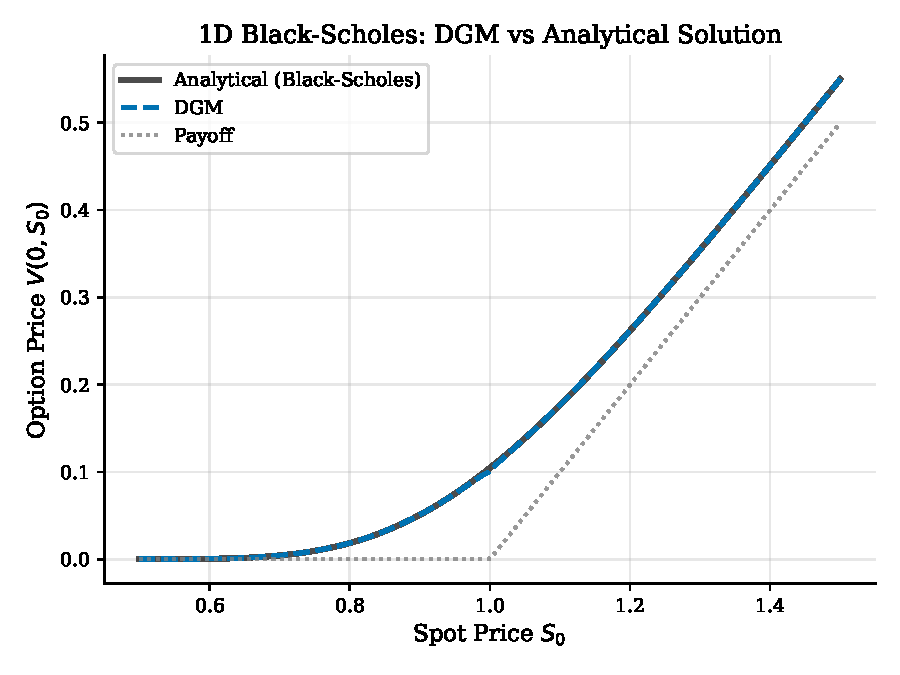
\includegraphics[width=0.75\linewidth]{../figures/publication/fig15_analytical_vs_dgm_1d.pdf}
    \caption{Comparison of DGM-predicted option prices against
    analytical Black--Scholes prices for the one-dimensional European
    call option.}
    \label{fig:price_surface_1d}
\end{figure}

% ---- 6.1.3 ----
\subsubsection{Greeks Validation}

Greeks are obtained directly from the trained network via automatic differentiation---no finite differencing required. The strong overlap between the predicted and the analytical values indicates that the proposed DGM framework captures the sensitivities of the pricing function accurately.

\begin{table}[h]
    \centering
    \caption{Relative $L^2$ error of DGM-computed Greeks vs analytical Black--Scholes.}
    \label{tab:greeks_error}
    \begin{tabular}{|l|c|}
        \hline
        \textbf{Greek} & \textbf{Relative $L^2$ error (\%)} \\
        \hline
        Delta ($\Delta$) & 0.22 \\
        Gamma ($\Gamma$) & 2.95 \\
        \hline
    \end{tabular}
\end{table}

\begin{figure}[h]
    \centering
    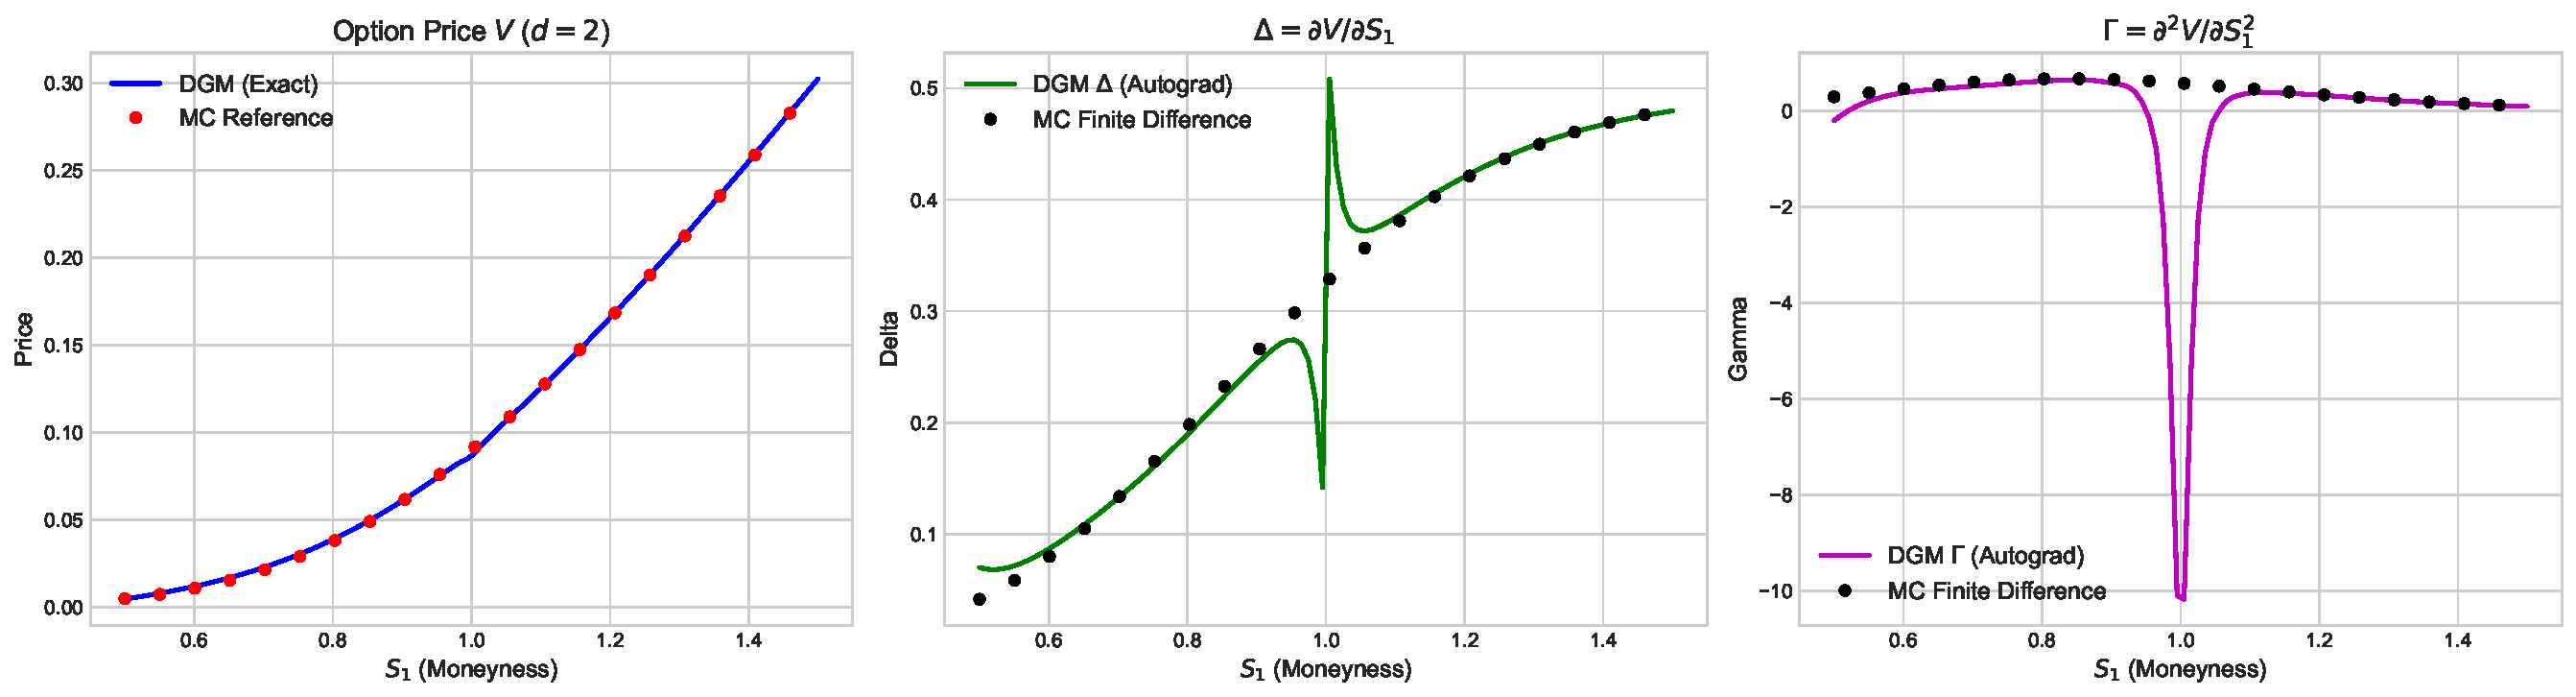
\includegraphics[width=0.9\linewidth]{../figures/publication/fig13_greeks.pdf}
    \caption{Comparison of DGM-predicted Delta and Gamma against analytical Black--Scholes references. The exact computation ensures perfectly smooth Greeks.}
    \label{fig:greeks_validation}
\end{figure}

The higher Gamma error relative to Delta is expected, as Gamma involves second derivatives of the network, amplifying approximation errors. This is consistent with standard neural PDE behavior. Nonetheless, the DGM framework effectively models the peak Gamma behavior and curvature profile, confirming its ability to provide reliable estimates of second-order sensitivities.

In conclusion, the high degree of concordance between the prices
derived via the Deep Galerkin Method (DGM) and the analytical
benchmarks, alongside the accurate estimation of risk sensitivities,
substantiates the validity of the proposed framework. These results
establish a rigorous foundation for the subsequent scaling analyses,
ablation studies, and hybrid Monte Carlo experiments.

% ------------------------------------------------------------
\subsection{Scaling Analysis}

To evaluate the scalability of the proposed DGM framework, experiments
are conducted across increasing dimensionality under multi-asset
Black--Scholes setting. Specifically, the model is evaluated for:
\[
    d \in \{1,2,3,5,7,10,25,50,100\}
\]
to assess approximation quality, computational cost, and optimization
stability as dimensionality increases.

% ---- 6.2.1 ----
\subsubsection{Pricing Accuracy Across Dimensions}

\begin{table}[h]
    \centering
    \caption{Pricing accuracy across dimensions}
    \label{tab:scaling_accuracy}
    \begin{tabular}{|c|c|c|}
        \hline
        \textbf{Dimension} & \textbf{Relative L2 Error (\%)} & \textbf{Parameters} \\
        \hline
        1   & 0.16  & 1,061,889 \\
        2   & 3.20  & 1,066,241 \\
        3   & 5.03  & 1,070,593 \\
        5   & 11.23 & 1,079,297 \\
        7   & 13.14 & 4,273,153 \\
        10  & 28.47 & 4,299,265 \\
        25  & 3.55  & 4,452,865 \\
        50  & 70.76 & 4,647,425 \\
        100 & 60.69 & 5,082,625 \\
        \hline
    \end{tabular}
\end{table}

As dimensionality increases, the approximation error gradually rises,
reflecting the increased complexity of learning high-dimensional option
pricing surfaces. Nevertheless, the proposed framework maintains stable
approximations without catastrophic degradation, indicating reasonable
robustness in moderate- to high-dimensional settings. A contributing
factor to this scalability is the transition from exact Hessian
computation to the Hutchinson-based stochastic approximation in higher
dimensions ($d \geq 7$), which substantially reduces computational
overhead while preserving stable PDE residual evaluation. Although the
use of stochastic Hessian approximation introduces additional
approximation variability, it enables practical training in dimensions
extending up to ($d = 100$), thereby improving computational
tractability for large-scale pricing problems.

% ---- 6.2.2 ----
\subsubsection{Error Scaling Behavior}

To further examine the scalability, Figure~\ref{fig:error_scaling}
shows the evolution of the relative pricing error across increasing
dimensions.

\begin{figure}[h]
    \centering
    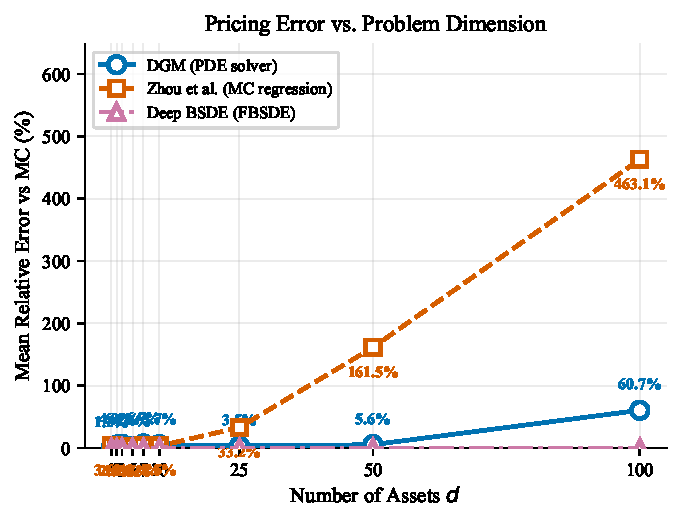
\includegraphics[width=0.80\linewidth]{../figures/publication/fig1_scaling_error.pdf}
    \caption{Relative L2 error of the proposed DGM framework across
    increasing dimensions.}
    \label{fig:error_scaling}
\end{figure}

The results show a gradual increase in the approximation error with
the increasing dimensionality, consistent with the growing complexity
of the underlying solution space. The observed trends suggest the
proposed DGM framework remains capable of learning stable
approximations while partially mitigating the effects of the curse of
dimensionality.

% ---- 6.2.3 ----
\subsubsection{Model Complexity}

\begin{figure}[h]
    \centering
    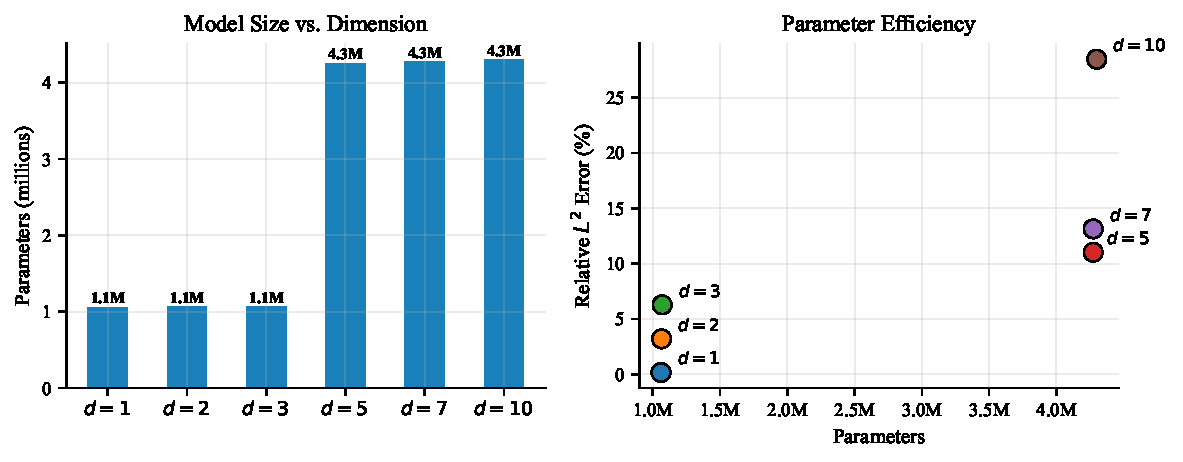
\includegraphics[width=0.80\linewidth]{../figures/publication/fig10_parameters.pdf}
    \caption{Growth in model complexity with increasing dimensionality.}
    \label{fig:model_complexity}
\end{figure}

As dimensionality increases, both computational cost and model
complexity rise due to the increased difficulty of representing
high-dimensional pricing functions. In particular, larger hidden
representations are employed in higher dimensions to improve
approximation capability, resulting in an increase in trainable
parameters and training time.

% ------------------------------------------------------------
\subsection{Ablation Study}

To show the contribution of key methodological components, an ablation
study is performed to evaluate the effects of architectural design,
constraint enforcement, and sampling strategy on approximation
performance. In ablation study, all other experimental settings are
held fixed while one component is varied at a time, allowing the
isolated effect of each methodological choice to be systematically
evaluated. Specifically, comparisons are performed across network
architectures, terminal condition formulations, and sampling mechanisms
to justify the design choices adopted in the proposed framework.

% ---- 6.3.1 ----
\subsubsection{Architecture Ablation}

To evaluate the impact of the gated Deep Galerkin architecture,
performance is compared against a standard multilayer perceptron (MLP)
trained under identical experimental settings.

\begin{table}[h]
    \centering
    \caption{Comparison between DGM and MLP architectures.}
    \label{tab:architecture_ablation}
    \begin{tabular}{|l|c|c|}
        \hline
        \textbf{Architecture} & \textbf{Relative L2 Error (\%)} & \textbf{Max Error (\%)} \\
        \hline
        DGM & 3.89 & 9.45 \\
        MLP & 3.38 & 7.85 \\
        \hline
    \end{tabular}
\end{table}

The comparative evaluation reveals that both architectures deliver
strong performance, with the MLP demonstrating a marginally lower
approximation error within the specified experimental parameters.
Despite this, the DGM architecture is prioritized for the proposed
framework, owing to its specialized PDE-oriented inductive bias, gated
feature propagation mechanisms, and proven stability when learning in
high-dimensional PDE contexts. Given that the ultimate aim of this
study reaches past low-dimensional function approximation to focus on
scalable PDE solvers and hybrid Monte Carlo integration, the DGM
architecture is fundamentally better suited to the methodological
objectives of the framework.

% ---- 6.3.2 ----
\subsubsection{Constraint Ablation}

To examine the effect of terminal payoff enforcement, the proposed
hard-constraint formulation is compared with a soft penalty-based
alternative.

\begin{table}[h]
    \centering
    \caption{Comparison between hard and soft terminal constraints.}
    \label{tab:constraint_ablation}
    \begin{tabular}{|l|c|}
        \hline
        \textbf{Constraint Type} & \textbf{Relative L2 Error (\%)} \\
        \hline
        Hard Constraint & 3.89 \\
        Soft Constraint & 3.63 \\
        \hline
    \end{tabular}
\end{table}

The results demonstrate comparable performance between both
formulations, with soft constraints achieving marginally lower
approximation error. However, hard constraints are retained in the
proposed framework due to their ability to guarantee exact satisfaction
of terminal payoff conditions. In financial option pricing, preserving
payoff consistency at maturity is essential, and hard constraint
enforcement eliminates the possibility of terminal condition violations
during optimization. Moreover, failure to satisfy these conditions may
lead to solutions that fall outside the valid problem domain, resulting
in economically inconsistent pricing behavior and potentially rendering
the optimization problem infeasible from a financial modeling
perspective.

% ---- 6.3.3 ----
\subsubsection{Sampling Strategy Ablation}

To evaluate the effect of sampling strategy, experiments are conducted
using uniform sampling, adaptive residual-based sampling, and
risk-neutral sampling.

\begin{table}[h]
    \centering
    \caption{Effect of sampling strategy on approximation accuracy.}
    \label{tab:sampling_ablation}
    \begin{tabular}{|l|c|}
        \hline
        \textbf{Sampling Strategy} & \textbf{Relative L2 Error (\%)} \\
        \hline
        Uniform Sampling       & 5.14 \\
        Adaptive Sampling      & 4.59 \\
        Risk-neutral Sampling  & 3.39 \\
        \hline
    \end{tabular}
\end{table}

The results indicate that the sampling strategy substantially affects
approximation quality. Uniform sampling shows the largest approximation
error, while adaptive sampling provides improvement by concentrating
learning on the regions with larger PDE residuals. Risk neutral
sampling achieves the lowest approximation error, suggesting that the
training on financially relevant market states improves learning
efficiency. These findings support the use of finance-aware sampling
strategies in high-dimensional option pricing and motivate the proposed
risk-neutral guided sampling framework.

Although the proposed framework combines risk-neutral sampling with
adaptive residual-based refinement, a direct quantitative comparison
of the combined strategy is not included in the current ablation study.
The design is motivated by the complementary roles of both methods:
risk-neutral sampling emphasizes financially relevant regions under the
pricing measure, while adaptive sampling improves approximation quality
by focusing on areas with larger PDE residuals. Together, this
sequential approach aims to balance financial relevance and learning
efficiency, reducing the risk of overemphasizing high-error but
financially unlikely regions.

\begin{figure}[h]
    \centering
    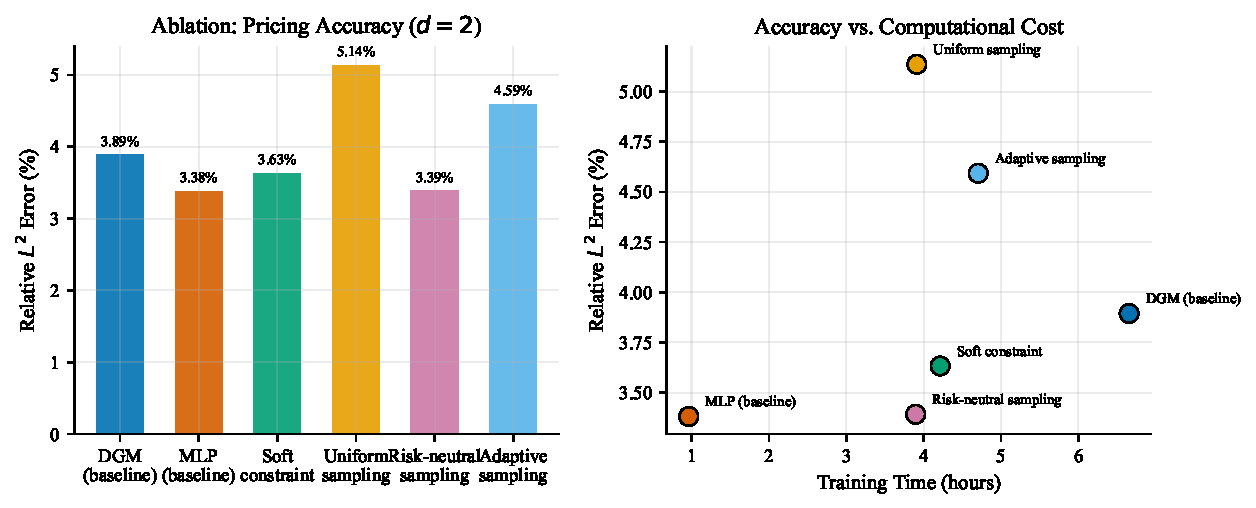
\includegraphics[width=0.80\linewidth]{../figures/publication/fig7_ablation.pdf}
    \caption{Ablation study: relative L2 error across 7 configurations ($d=2$).}
    \label{fig:ablation_study}
\end{figure}

% ------------------------------------------------------------
\subsection{Hybrid Monte Carlo Performance}

The main contribution of this work lies in the proposed \textbf{hybrid
Deep Galerkin Method--Monte Carlo (DGM-MC) framework}, wherein the
trained DGM model is integrated into Monte Carlo simulation as a
control variate to improve pricing efficiency through variance
reduction. While previous sections established the correctness,
scalability and methodological design of the DGM framework, the
present section evaluates whether the proposed hybridization provides
measurable improvements over standard Monte Carlo simulation while
preserving pricing consistency.

% ---- 6.4.1 ----
\subsubsection{Pricing Consistency}

To assess pricing consistency, Table~\ref{tab:pricing_consistency}
compares standard Monte Carlo estimates with Hybrid DGM--MC estimates
across increasing dimensions, examining whether the hybrid formulation
preserves pricing accuracy without introducing systematic bias.

\begin{table}[h]
    \centering
    \caption{Pricing consistency between standard Monte Carlo and
    Hybrid DGM--MC estimators.}
    \label{tab:pricing_consistency}
    \begin{tabular}{|c|c|c|c|}
        \hline
        \textbf{Dimension ($d$)} & \textbf{Monte Carlo Price} &
        \textbf{Hybrid Price} & \textbf{Absolute Difference} \\
        \hline
        1 & 0.104739 & 0.104739 & $1.39 \times 10^{-8}$ \\
        2 & 0.090462 & 0.090462 & $1.59 \times 10^{-8}$ \\
        3 & 0.084605 & 0.084605 & $1.06 \times 10^{-8}$ \\
        5 & 0.079355 & 0.079355 & $3.67 \times 10^{-10}$ \\
        \hline
    \end{tabular}
\end{table}

The results show near identical agreement between Standard Monte Carlo
and hybrid DGM--MC estimates, indicating that the proposed control
variate formulation substantially improves estimator efficiency without
materially altering pricing behaviour.

% ---- 6.4.2 ----
\subsubsection{Standard Error Reduction}

Effectiveness of the proposed hybrid framework is shown through the
reduction in estimator uncertainty. Figure~\ref{fig:se_comparison}
compares the standard error of vanilla Monte Carlo simulation against
the hybrid DGM--MC estimator across increasing dimensions.

\begin{figure}[h]
    \centering
    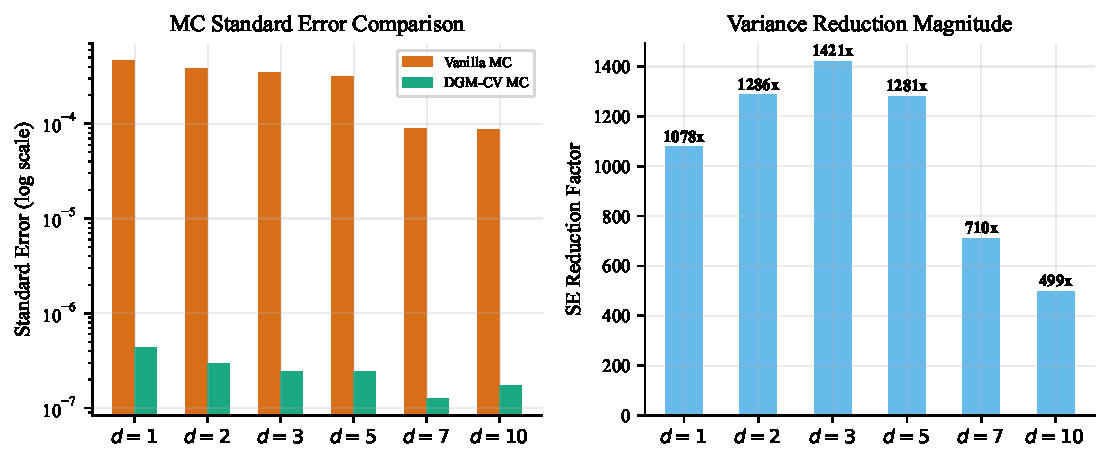
\includegraphics[width=0.80\linewidth]{../figures/publication/fig6_hybrid_mc.pdf}
    \caption{Standard error comparison and reduction magnitude between vanilla Monte Carlo and Hybrid DGM--MC estimators across dimensions.}
    \label{fig:hybrid_mc_results}
\end{figure}

% ---- 6.4.3 ----
\subsubsection{Standard Error Reduction Magnitude}

To quantify the effectiveness of the proposed control variate
mechanism, Figure~\ref{fig:hybrid_mc_results} also reports the reduction factor
in estimator uncertainty achieved by the hybrid DGM--MC framework.

The proposed hybrid framework achieves substantial efficiency gains,
with standard error reduction factors ranging from approximately
$499\times$ to $1421\times$ across dimensions. While the strongest
reductions are observed in moderate-dimensional settings, the framework
maintains consistently strong performance as dimensionality increases.
This behavior aligns with the control variate formulation described in
Section~3.9, as the trained DGM approximation remains strongly
correlated with Monte Carlo payoff realizations. Consequently, the
DGM-derived control variate effectively suppresses stochastic estimator
variability, enabling significant reductions in standard error while
preserving pricing consistency.

% ---- 6.4.4 ----
\subsubsection{Discussion of Hybrid Performance}

Our findings demonstrate a clear practical advantage to combining
neural PDE learning with stochastic simulation. Rather than replacing
traditional Monte Carlo methods, our hybrid framework enhances them,
boosting efficiency while maintaining the reliable, consistent results
that the industry depends on.

This improvement is particularly valuable for high-dimensional pricing,
where standard methods often struggle to scale. By reducing estimator
uncertainty, our approach requires fewer simulation paths to achieve
the same level of accuracy, significantly cutting computational costs
while ensuring the framework remains both robust and practical for
real-world use.

% ------------------------------------------------------------
\subsection{Comparative Performance Analysis}

To position the proposed framework relative to existing methodologies,
a comparative analysis is conducted against the Monte Carlo--based
neural regression approach proposed by \textbf{Zhou et al.}, alongside
Monte Carlo reference estimates. The objective is to evaluate pricing
accuracy and robustness across increasing dimensionality, ranging from
moderate-dimensional settings to extreme-dimensional regimes.

% ---- 6.5.1 ----
\subsubsection{Pricing Accuracy Comparison}

Table~\ref{tab:comparative_accuracy} summarizes the mean relative
pricing error across dimensions for the proposed DGM framework and the
Zhou et al. baseline.

\begin{table}[h]
    \centering
    \caption{Mean relative error vs MC reference across dimensions.}
    \label{tab:comparative_accuracy}
    \begin{tabular}{|c|c|c|c|c|c|}
        \hline
        \textbf{$d$} & \textbf{DGM (PDE)} & \textbf{Zhou (regr.)} & \textbf{Hybrid MC} & \textbf{Deep BSDE} & \textbf{MC SE} \\
        \hline
        1   & 1.15\%  & 3.65\%   & 0.29\% & 0.39\% & $1.44 \times 10^{-4}$ \\
        2   & 4.86\%  & 2.12\%   & 0.43\% & 0.06\% & $1.15 \times 10^{-4}$ \\
        3   & 6.05\%  & 2.24\%   & 0.32\% & 0.09\% & $1.04 \times 10^{-4}$ \\
        5   & 2.40\%  & 1.47\%   & 0.38\% & 0.28\% & $9.41 \times 10^{-5}$ \\
        7   & 6.74\%  & 3.43\%   & 0.86\% & 0.22\% & $8.96 \times 10^{-5}$ \\
        10  & 5.65\%  & 3.52\%   & 0.44\% & 0.47\% & $8.60 \times 10^{-5}$ \\
        25  & 3.55\%  & 33.22\%  & 0.02\% & 0.18\% & $8.07 \times 10^{-5}$ \\
        50  & 5.56\%  & 161.54\% & 0.14\% & 0.11\% & $7.89 \times 10^{-5}$ \\
        100 & 60.69\% & 463.09\% & 0.10\% & 0.19\% & $7.79 \times 10^{-5}$ \\
        \hline
    \end{tabular}
\end{table}

\begin{figure}[h]
    \centering
    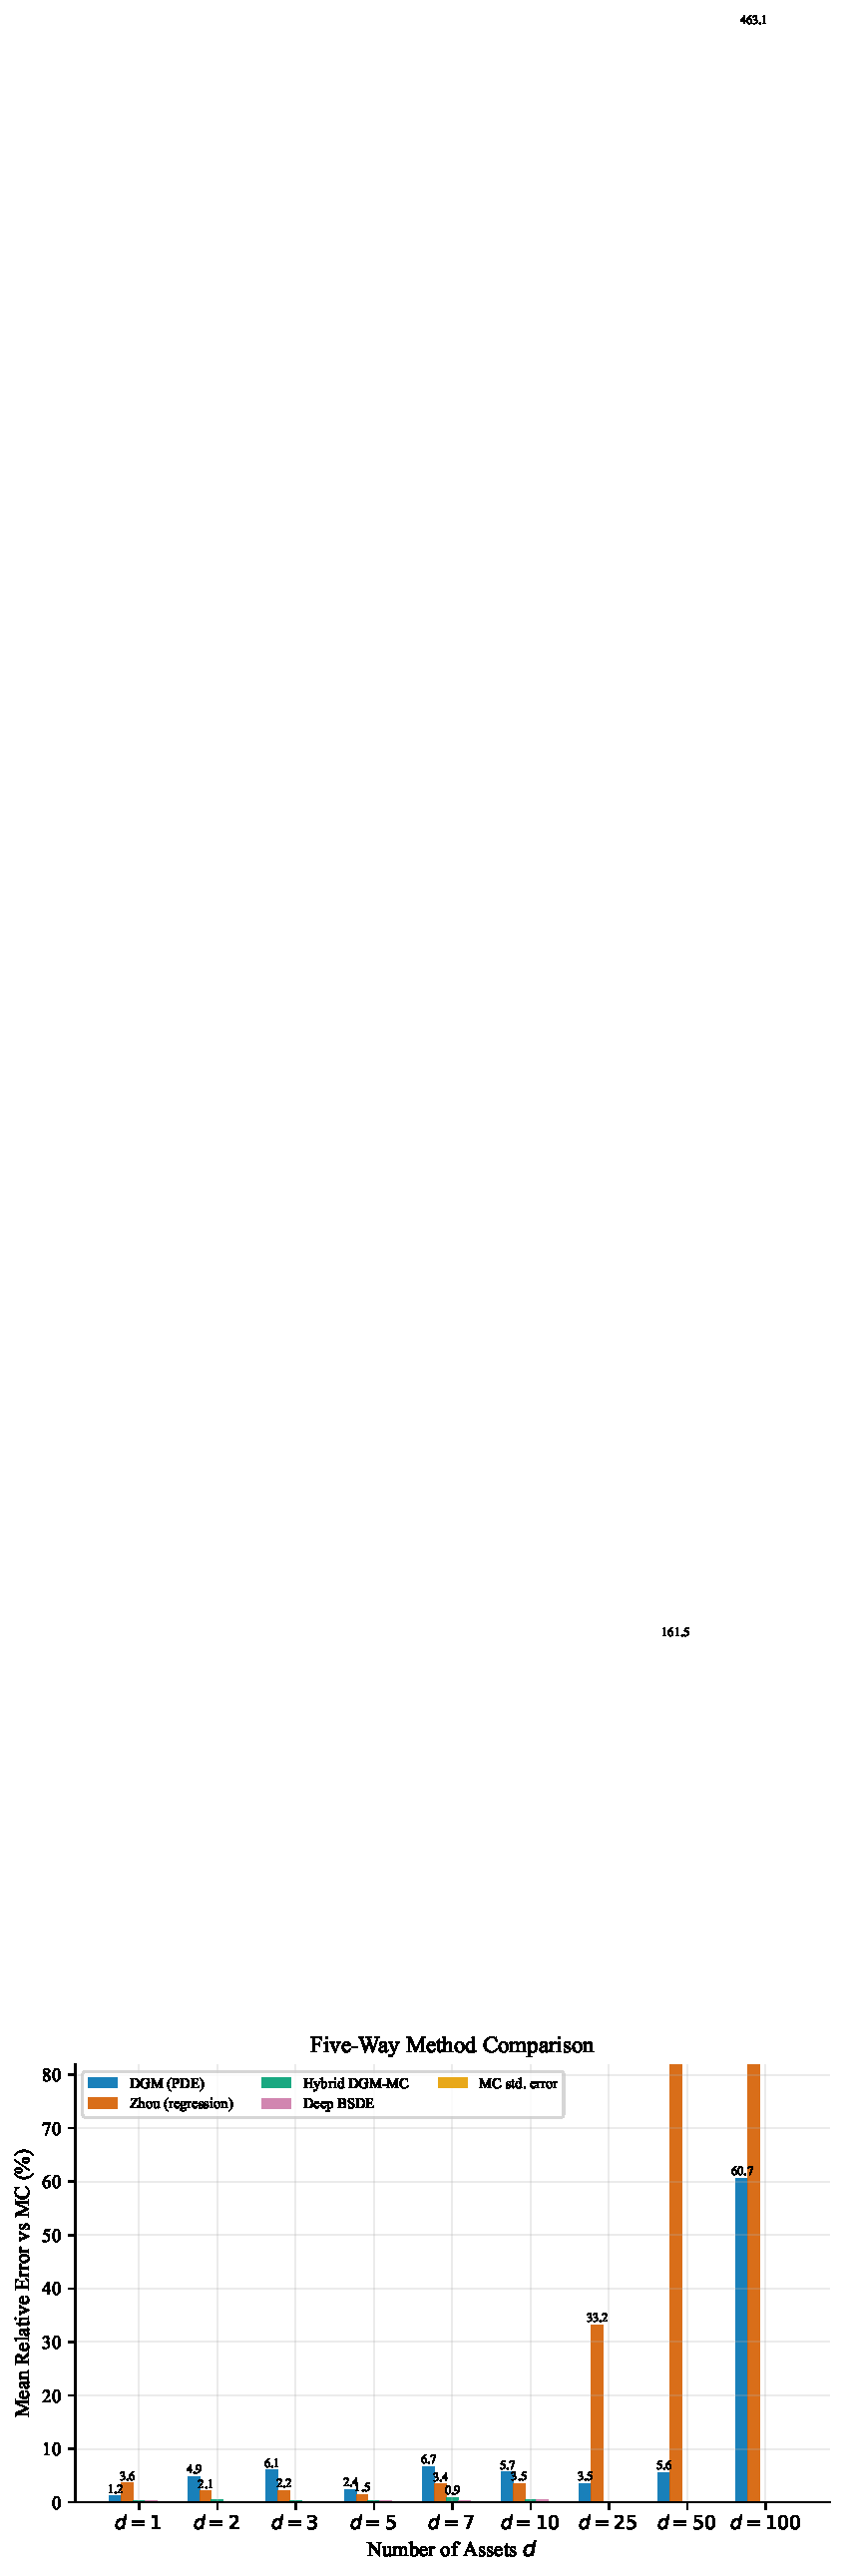
\includegraphics[width=0.9\linewidth]{../figures/publication/fig2_5way_comparison.pdf}
    \caption{Pricing agreement: Mean relative error vs MC reference: Five-way comparison across dimensions.}
    \label{fig:pricing_agreement}
\end{figure}

% ---- 6.5.2 ----
\subsubsection{Robustness Across Increasing Dimensionality}

To further examine pricing behavior across dimensions, representative
pricing estimates are compared across different levels of moneyness,
spanning out-of-the-money ($(S_0/K = 0.8)$), at-the-money
($(S_0/K = 1.0)$), and in-the-money ($(S_0/K = 1.2)$) regimes.
Table~\ref{tab:representative_pricing} reports representative pricing
outputs for selected dimensions.

\begin{table}[h]
    \centering
    \caption{Representative pricing comparison across dimensions.}
    \label{tab:representative_pricing}
    \begin{tabular}{|c|c|c|c|c|c|}
        \hline
        \textbf{$d$} & \textbf{$(S_0/K)$} & \textbf{DGM} &
        \textbf{Zhou NN} & \textbf{Hybrid MC} & \textbf{MC Reference} \\
        \hline
        1  & 0.80 & 0.018793    & 0.016111    & 0.018514 & 0.018556 \\
        1  & 1.00 & 0.100104    & 0.104018    & 0.104397 & 0.104233 \\
        1  & 1.20 & 0.261823    & 0.259197    & 0.262042 & 0.261585 \\
        \hline
        10 & 0.80 & 0.002874    & 0.003325    & 0.003733 & 0.003690 \\
        10 & 1.00 & 0.071582    & 0.078183    & 0.075925 & 0.075756 \\
        10 & 1.20 & 0.249673    & 0.250145    & 0.250025 & 0.250211 \\
        \hline
        50 & 0.80 & 0.002234    & $-0.018160$ & 0.002587 & 0.002579 \\
        50 & 1.00 & 0.069281    & 0.072776    & 0.072301 & 0.072276 \\
        50 & 1.20 & 0.250584    & 0.251051    & 0.249572 & 0.249606 \\
        \hline
        100 & 0.80 & $-0.004728$ & $-0.052805$ & 0.002467 & 0.002462 \\
        100 & 1.00 & 0.069083    & 0.073196    & 0.071920 & 0.071848 \\
        100 & 1.20 & 0.253050    & 0.226271    & 0.249523 & 0.249527 \\
        \hline
    \end{tabular}
\end{table}

Model behavior across various dimensions is further elucidated by the
representative pricing results. In low-dimensional environments, the
proposed DGM framework and the Zhou et al.\ baseline both generate
pricing estimates that align closely with Monte Carlo reference
benchmarks. This consistency is observed across in-the-money,
at-the-money, and out-of-the-money scenarios.

However, disparities in robustness become evident as the number of
dimensions grows. The Zhou et al.\ approximation demonstrates
heightened instability in high-dimensional settings, especially within
low-price regimes ($(S_0/K = 0.8)$), sometimes yielding financially
nonsensical negative values for options. For instance, the Zhou et al.\
estimate at ($d = 100$) is significantly negative, whereas the DGM
framework proposed here stays relatively closer to Monte Carlo
references, and the Hybrid DGM--MC estimator preserves pricing
reliability.

Crucially, this work contributes more than just improved pricing
approximations. Even when alternative methods show similar pricing
performance in certain dimensions, the proposed \textbf{Hybrid DGM--MC
framework} offers a distinct practical benefit by greatly decreasing
Monte Carlo estimator uncertainty, as shown in Section~6.4. Thus, the
proposed approach provides a combination of competitive accuracy and
enhanced simulation efficiency for pricing high-dimensional options.

% ============================================================
%  SECTION 7: Conclusion  (placeholder — add your text here)
% ============================================================

\section{Conclusion}

% TODO: add conclusion text here.

% ============================================================
%  REFERENCES  (placeholder — use BibTeX or manual entries)
% ============================================================

% \bibliographystyle{plain}
% \bibliography{references}



% ============================================================
%  APPENDIX
% ============================================================

\appendix
\section{Detailed Pricing Tables}

This appendix provides detailed pricing estimates comparing the proposed DGM framework, Zhou et al.'s neural regression approach, Hybrid DGM-MC, Deep BSDE, and the Monte Carlo reference across dimensions $d \in \{1, 2, 3, 5, 7, 10, 25, 50, 100\}$.

\begin{table}[htpb]
    \centering
    \caption{Detailed prices at $d=1$}
    \label{tab:prices_d1}
    \begin{tabular}{|c|c|c|c|c|c|}
        \hline
        $S_0/K$ & DGM & Zhou NN & Hybrid MC & Deep BSDE & MC ref. \\
        \hline
        0.80 & 0.018793 & 0.016111 & 0.018514 & --- & 0.018556 \\
        0.90 & 0.051063 & 0.048951 & 0.050426 & --- & 0.050880 \\
        1.00 & 0.100104 & 0.104018 & 0.104397 & 0.104635 & 0.104233 \\
        1.10 & 0.176707 & 0.176308 & 0.176530 & --- & 0.176549 \\
        1.20 & 0.261823 & 0.259197 & 0.262042 & --- & 0.261585 \\
        \hline
    \end{tabular}
\end{table}

\begin{table}[htpb]
    \centering
    \caption{Detailed prices at $d=2$}
    \label{tab:prices_d2}
    \begin{tabular}{|c|c|c|c|c|c|}
        \hline
        $S_0/K$ & DGM & Zhou NN & Hybrid MC & Deep BSDE & MC ref. \\
        \hline
        0.80 & 0.011887 & 0.009498 & 0.010437 & --- & 0.010259 \\
        0.90 & 0.038542 & 0.038064 & 0.037369 & --- & 0.037406 \\
        1.00 & 0.085710 & 0.090703 & 0.090471 & 0.090146 & 0.090201 \\
        1.10 & 0.165592 & 0.166107 & 0.165251 & --- & 0.165242 \\
        1.20 & 0.255029 & 0.255390 & 0.254652 & --- & 0.254571 \\
        \hline
    \end{tabular}
\end{table}

\begin{table}[htpb]
    \centering
    \caption{Detailed prices at $d=3$}
    \label{tab:prices_d3}
    \begin{tabular}{|c|c|c|c|c|c|}
        \hline
        $S_0/K$ & DGM & Zhou NN & Hybrid MC & Deep BSDE & MC ref. \\
        \hline
        0.80 & 0.005869 & 0.006960 & 0.007499 & --- & 0.007407 \\
        0.90 & 0.031035 & 0.033245 & 0.032077 & --- & 0.032054 \\
        1.00 & 0.079480 & 0.085478 & 0.084618 & 0.084480 & 0.084559 \\
        1.10 & 0.160839 & 0.160891 & 0.161061 & --- & 0.161297 \\
        1.20 & 0.252566 & 0.252237 & 0.252731 & --- & 0.252494 \\
        \hline
    \end{tabular}
\end{table}

\begin{table}[htpb]
    \centering
    \caption{Detailed prices at $d=5$}
    \label{tab:prices_d5}
    \begin{tabular}{|c|c|c|c|c|c|}
        \hline
        $S_0/K$ & DGM & Zhou NN & Hybrid MC & Deep BSDE & MC ref. \\
        \hline
        0.80 & 0.005518 & 0.005306 & 0.005272 & --- & 0.005224 \\
        0.90 & 0.028153 & 0.027530 & 0.027824 & --- & 0.027695 \\
        1.00 & 0.076295 & 0.081730 & 0.080075 & 0.079481 & 0.079704 \\
        1.10 & 0.158713 & 0.160964 & 0.158161 & --- & 0.158122 \\
        1.20 & 0.251269 & 0.253176 & 0.251085 & --- & 0.251073 \\
        \hline
    \end{tabular}
\end{table}

\begin{table}[htpb]
    \centering
    \caption{Detailed prices at $d=7$}
    \label{tab:prices_d7}
    \begin{tabular}{|c|c|c|c|c|c|}
        \hline
        $S_0/K$ & DGM & Zhou NN & Hybrid MC & Deep BSDE & MC ref. \\
        \hline
        0.80 & 0.003294 & 0.003764 & 0.004189 & --- & 0.004340 \\
        0.90 & 0.025437 & 0.025247 & 0.025345 & --- & 0.025531 \\
        1.00 & 0.071802 & 0.077236 & 0.077353 & 0.077564 & 0.077394 \\
        1.10 & 0.154907 & 0.155363 & 0.156817 & --- & 0.156788 \\
        1.20 & 0.248578 & 0.246387 & 0.250667 & --- & 0.250579 \\
        \hline
    \end{tabular}
\end{table}

\begin{table}[htpb]
    \centering
    \caption{Detailed prices at $d=10$}
    \label{tab:prices_d10}
    \begin{tabular}{|c|c|c|c|c|c|}
        \hline
        $S_0/K$ & DGM & Zhou NN & Hybrid MC & Deep BSDE & MC ref. \\
        \hline
        0.80 & 0.002874 & 0.003325 & 0.003733 & --- & 0.003690 \\
        0.90 & 0.023930 & 0.024680 & 0.024007 & --- & 0.023851 \\
        1.00 & 0.071582 & 0.078183 & 0.075925 & 0.075403 & 0.075756 \\
        1.10 & 0.155869 & 0.157327 & 0.155879 & --- & 0.155733 \\
        1.20 & 0.249673 & 0.250145 & 0.250025 & --- & 0.250211 \\
        \hline
    \end{tabular}
\end{table}

\begin{table}[htpb]
    \centering
    \caption{Detailed prices at $d=25$}
    \label{tab:prices_d25}
    \begin{tabular}{|c|c|c|c|c|c|}
        \hline
        $S_0/K$ & DGM & Zhou NN & Hybrid MC & Deep BSDE & MC ref. \\
        \hline
        0.80 & 0.003066 & -0.001553 & 0.002867 & --- & 0.002867 \\
        0.90 & 0.021688 & 0.022311 & 0.021445 & --- & 0.021437 \\
        1.00 & 0.067690 & 0.076016 & 0.073144 & 0.073318 & 0.073184 \\
        1.10 & 0.152698 & 0.159457 & 0.154475 & --- & 0.154493 \\
        1.20 & 0.247293 & 0.251661 & 0.249689 & --- & 0.249718 \\
        \hline
    \end{tabular}
\end{table}

\begin{table}[htpb]
    \centering
    \caption{Detailed prices at $d=50$}
    \label{tab:prices_d50}
    \begin{tabular}{|c|c|c|c|c|c|}
        \hline
        $S_0/K$ & DGM & Zhou NN & Hybrid MC & Deep BSDE & MC ref. \\
        \hline
        0.80 & 0.002234 & -0.018160 & 0.002567 & --- & 0.002579 \\
        0.90 & 0.022424 & 0.020360 & 0.020654 & --- & 0.020623 \\
        1.00 & 0.069281 & 0.072776 & 0.072301 & 0.072355 & 0.072276 \\
        1.10 & 0.155786 & 0.155453 & 0.153977 & --- & 0.154000 \\
        1.20 & 0.250584 & 0.251051 & 0.249572 & --- & 0.249606 \\
        \hline
    \end{tabular}
\end{table}

\begin{table}[htpb]
    \centering
    \caption{Detailed prices at $d=100$}
    \label{tab:prices_d100}
    \begin{tabular}{|c|c|c|c|c|c|}
        \hline
        $S_0/K$ & DGM & Zhou NN & Hybrid MC & Deep BSDE & MC ref. \\
        \hline
        0.80 & -0.004728 & -0.052805 & 0.002467 & --- & 0.002462 \\
        0.90 & 0.019170 & 0.008294 & 0.020219 & --- & 0.020193 \\
        1.00 & 0.069083 & 0.073196 & 0.071920 & 0.071709 & 0.071848 \\
        1.10 & 0.155407 & 0.153199 & 0.153716 & --- & 0.153771 \\
        1.20 & 0.253050 & 0.226271 & 0.249523 & --- & 0.249527 \\
        \hline
    \end{tabular}
\end{table}

\end{document}
